\section{Multigrid Method with Augmented Variables}
Condition of equation~\ref{equ:local_metric}, states that prolongation operator must correctly interpolate error vectors $\mathbf{e}$ that are in the Null space of the local matrix $\mathbf{A}_i$. Here I will give without prove that standard multi-linear interpolation satisfies this condition for both elasticity and Poisson problems, as it is used for homogeneous problems and proven to be effective. In section~\ref{sec:p_sparsity}, a sparsity condition for the prolongation operator was imposed to guarantee the sparsity of the coarse level operators. Considering Figure~\ref{fig:neighbor_ring}, that the fine node is interpolated from the edge adjacent two coarse nodes. For 3D elasticity, the two coarse nodes provides 6 equations in solving the local prolongation operator. Note that the Nullity of $\mathbf{A}_i$ is also 6. Which means there is only one prolongation operator satisfies the condition of equation~\ref{equ:local_metric}, and we know that the standard multi-linear interpolation satisfies this condition. Therefore:
\begin{lem}\label{lemma:linear_best} 
 Multi-linear interpolation is the \textbf{only} interpolation that can capture error vectors in the null space of local matrix $\mathbf{A}_i$ for fine nodes that are interpolated from only two coarse nodes in 3D elasticity problems.
\end{lem}
Given that the largest $M_{i,p}$ is the upper bound for the multigrid convergence rate, which means it is very difficult to improve the convergence over multi-linear interpolated multigrid while maintaining our sparsity constraints for the prolongation operator. In work \cite{dohrmann2007interpolation}, similar observations were made. By introducing additional degrees of freedom in the coarse grids, better solutions to equation~\ref{equ:local_metric} can be achieved. 
\subsection{Introducing Linearized Rotational Degrees of Freedom}
Similar to \cite{dohrmann2007interpolation}, we introduced linearized rotational degrees of freedom to the coarse grid to improve the quality of the prolongation operator. But different from it, given that our top level operator is matrix free as stated in chapter~\ref{Chapter:elasticity}, we can easily compute the element matrix on the top level and therefore avoiding the local null space analysis suggested in \cite{dohrmann2007interpolation}. First, I will introduce the additional linearized rotational DOF and their physical interpolation, then an algorithm will be provided for computing the solution given by theorem~\ref{theo:p_solution} with the extended DOF.
\begin{figure}[t]
\includegraphics[width=5cm]{BBMG/rotation.png}
\centering
\caption{A 2D example of a rotational degree of freedom $\theta$ and its physical interpolation in the case of interpolation fine node, marked blue, that is aligned with a coarse cell edge from two adjacent coarse nodes, marked yellow. Letters are associated names for the nodes. The solid lines indicates the deformed cells. The doted lines illustrated the undeformed cells.}
\label{fig:rotation_2D}
\end{figure}
Figure~\ref{fig:rotation_2D} illustrates the deformation created by the rotation DOF $\theta_L$ of node \textit{L} in 2D. The rotational degrees of freedom associated with node \textit{L}, namely $\theta_L$, is viewed influence the horizontal, and only the horizontal displacement of nodes \textit{LT} and \textit{LB}. If we write the the coarse DOF of node \textit{L}, displacements and rotation, denoted $\mathbf{u}^c_L$ for the local problem as:
$$
\mathbf{u}^c_L = \left(\begin{array}{c}u^c_L(x) \\ u^c_L(y) \\ u^c_L(\theta) \end{array}\right)
$$
The superscript $^c$ here indicates the DOF live on the coarse grid. Accordingly, the fine DOF of nodes \textit{LT}, \textit{L}, and \textit{LB}, then can be computed accordingly:
\begin{align*}
 \mathbf{u}^f_{LT} &= \left(\begin{array}{c} u^c_L(x) - u^c_L(\theta)h \\ * \end{array}\right) \\
 \mathbf{u}^f_{LT} &= \left(\begin{array}{c} u^c_L(x) \\ u^c_L(y) \end{array}\right) \\
 \mathbf{u}^f_{LB} &= \left(\begin{array}{c} u^c_L(x) + u^c_L(\theta)h \\ * \end{array}\right) 
\end{align*}
$h$ is the cell width. The symbol $*$ indicates that this DOF is not fixed for the local problem for interpolating the fine grid node values $\mathbf{u}^f_{C}$. Similarly we can write the right side nodal values as:
\begin{align*}
 \mathbf{u}^f_{RT} &= \left(\begin{array}{c} u^c_R(x) - u^c_R(\theta)h \\ * \end{array}\right) \\
 \mathbf{u}^f_{RT} &= \left(\begin{array}{c} u^c_R(x) \\ u^c_R(y) \end{array}\right) \\
 \mathbf{u}^f_{RB} &= \left(\begin{array}{c} u^c_R(x) + u^c_R(\theta)h \\ * \end{array}\right) 
\end{align*}
So if we rearrange the local matrix in equation~\ref{equ:local_matrix}, so that nodal values $\mathbf{u}^f_{C}$ first, then the other undetermined nodal values, and last, the eight determined nodal values we write as vector $\mathbf{u}^c$: 
$$
\mathbf{u}^c = \left(\mathbf{u}^f_{LT}(x), \mathbf{u}^f_{LT}(x), \mathbf{u}^f_{LT}(y), \mathbf{u}^f_{LB}(y),\mathbf{u}^f_{RT}(x), \mathbf{u}^f_{RT}(x), \mathbf{u}^f_{RT}(y), \mathbf{u}^f_{RB}(y)\right)
$$
We denote the rearranged local matrix as: 
 \begin{equation}
 \label{equ:matrix_split}
\mathbf{L}_i = \begin{bmatrix} 
\mathbf{L}_{ff} & \mathbf{L}_{fc} \\
\mathbf{L}_{cf} & \mathbf{L}_{cc}
\end{bmatrix}
\end{equation}
 Here $\mathbf{L}_{cc}$ is a $8\times8$ matrix, $\mathbf{L}_{ff}$ is of dimension $10\times10$. Based on theorem~\ref{theo:p_solution}, the fine nodal value vector $\mathbf{u}^f$ of size $10$ can than be computed as:
 \begin{equation}
 \mathbf{u}^f = -(\mathbf{L}_{ff})^{-1}\mathbf{L}_{fc}\mathbf{u}^c
 \end{equation} 
The local prolongation operator $\mathbf{P}_i$ is therefore:
 \begin{equation}
 \mathbf{P}_i = -(\mathbf{L}_{ff})^{-1}\mathbf{L}_{fc}
 \label{equ:edge_P_2D}
 \end{equation}
As we are using $\mathbf{L}_i$ instead of $\mathbf{L}^2_i$, our local convergence metric is therefore $M_{1,q}$. 
\subsection{Interpolation of Cell Centered Nodes in 2D}
Now that, we have interpolated the fine nodes that are aligned with the coarse cell edges. The next step is interpolating the fine nodes that are located in the center of the coarse cells, Figure~\ref{fig:embedded_interpolation}
\begin{figure}[t]
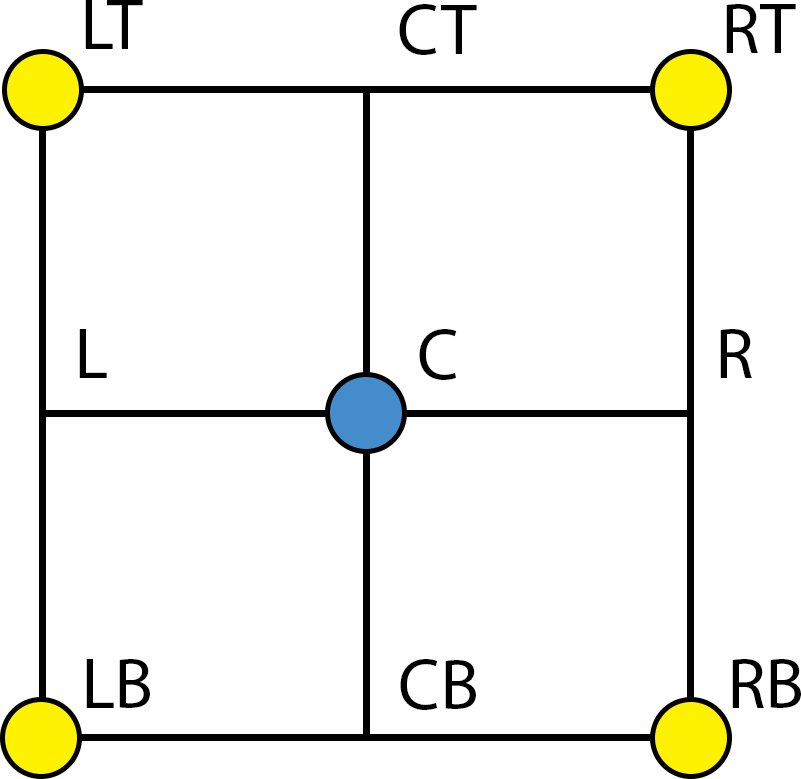
\includegraphics[width=5cm]{BBMG/Embeded_Interpolation}
\centering
\caption{Interpolation of a fine node, blue, that is in the center of a coarse cell. The coarse nodes are shaded in yellow. Each node is given a name.}
\label{fig:embedded_interpolation}
\end{figure}
Notice here that node \textit{CT} can be interpolated from node \textit{LT} and \textit{RT}. Similarly to node \textit{L},  \textit{R}, and \textit{CB}. As a matter of facts, that all the 8 neighbors of node \textit{C} can be interpolated. So, we can prolongate the node \textit{C} that has zero residual at the fine level. If $i$ is the index of node \textit{C}, and $\mathcal{N}_i$ is the set of nodes that are adjacent to node $i$, i.e.:
$$
\mathcal{N}_i = \{\textit{LB},\textit{CB},\textit{RB},\textit{L},\textit{R},\textit{LT},\textit{CT},\textit{RT}\}
$$
We can solve value of node $i$, denoted as $\mathbf{u}^f_i$ as:
\begin{equation}
\mathbf{L}_{ii}\mathbf{u}^f_i + \sum_{j \in \mathcal{N}_i}\mathbf{L}_{ij}\mathbf{P}_j\mathbf{u}^c = 0 
\end{equation}
Here $\mathbf{P}_j$ is the $j$th rows of the prolongation operator that computes the nodal values of $j$. In 2D, it is $2$ rows, and in 3D, it is three rows. So $\mathbf{P}_j\mathbf{u}^c$ computes the nodal value vector $\mathbf{u}^f_j$. $\mathbf{L}_{ij}$ is the stencil coefficient coupling node $j$ and $i$. It is a $2 \times 2$ matrix in 2D and $3 \times 3$ matrix in 3D. Therefore we can write the solution to $\mathbf{u}^f_i$ as:
\begin{equation}
\mathbf{u}^f_i = -\sum_{j \in \mathcal{N}_i}(\mathbf{L}_{ii})^{-1}\mathbf{L}_{ij}\mathbf{P}_j\mathbf{u}^c
\end{equation}
Therefore the prolongation operator for node $i$, $\mathbf{P}_i$ is then:
\begin{equation}
\mathbf{P}_i = -\sum_{j \in \mathcal{N}_i}(\mathbf{L}_{ii})^{-1}\mathbf{L}_{ij}\mathbf{P}_j
\end{equation}
\subsection{Interpolation of Fine Nodes that Coincide with a Coarse node in 2D}
This as the simplest case, same as a standard multi-linear interpolation, the fine node displacement are injected from the corresponding coarse node, while the rotational DOF are ignored.